\section{Cluster}\label{sec:cluster}
In this section, the cluster that will be doing the computations will be outlined. In \Cref{sec:clustersetup} the setup of the cluster and the available resources are listed, followed by a profile of the resource usage in \Cref{sec:profile}. In \Cref{sec:speedup} the speedup from using additional nodes for computations will be measured, both using several nodes and computation speed.

\subsection{Cluster Setup}\label{sec:clustersetup}

The cluster used for this work consist of four nodes, one master and three worker nodes. The master is master both in terms of cluster management on Spark and storage management on HDFS.\ Because of the limited resources for the project and small size of the cluster and dataset, some of the common fault tolerance functionality of Hadoop and Spark has not been employed. Most significantly, only one replication of data exist across HDFS, which naturally put large parts of the data at risk, however given the relatively small amount of machines and ease of access to new match data, we chose to prioritise data volume over fault tolerance. There are two unique setups of the nodes which can be seen in \Cref{tab:setups}.
\begin{table}[!htb]
  \centering
  \begin{tabular}{|r|ccc|}
    \hline
      & CPU & Storage & Memory \\\hline
    Setup 1 & Dual core intel e8400 3Ghz & 220 GB 7200 RPM & 4GB DDR2 \\
    Setup 2 & Quad core intel q9400 2.66Ghz & 220 GB 7200 RPM & 8GB DDR2 \\\hline
  \end{tabular}
  \caption{The different node setups}\label{tab:setups}
\end{table}

Where the master and one worker node has a dual core and the two remaining worker nodes have the quad cores. The machines are linked together using a switch capable of 200Mbit pr port, which sets a potential one-way bandwidth of 12.5MB/s pr machine. The physical setup of the cluster can be seen in \Cref{fig:clustersetup}.

\begin{figure}[!htb]
  \centering
    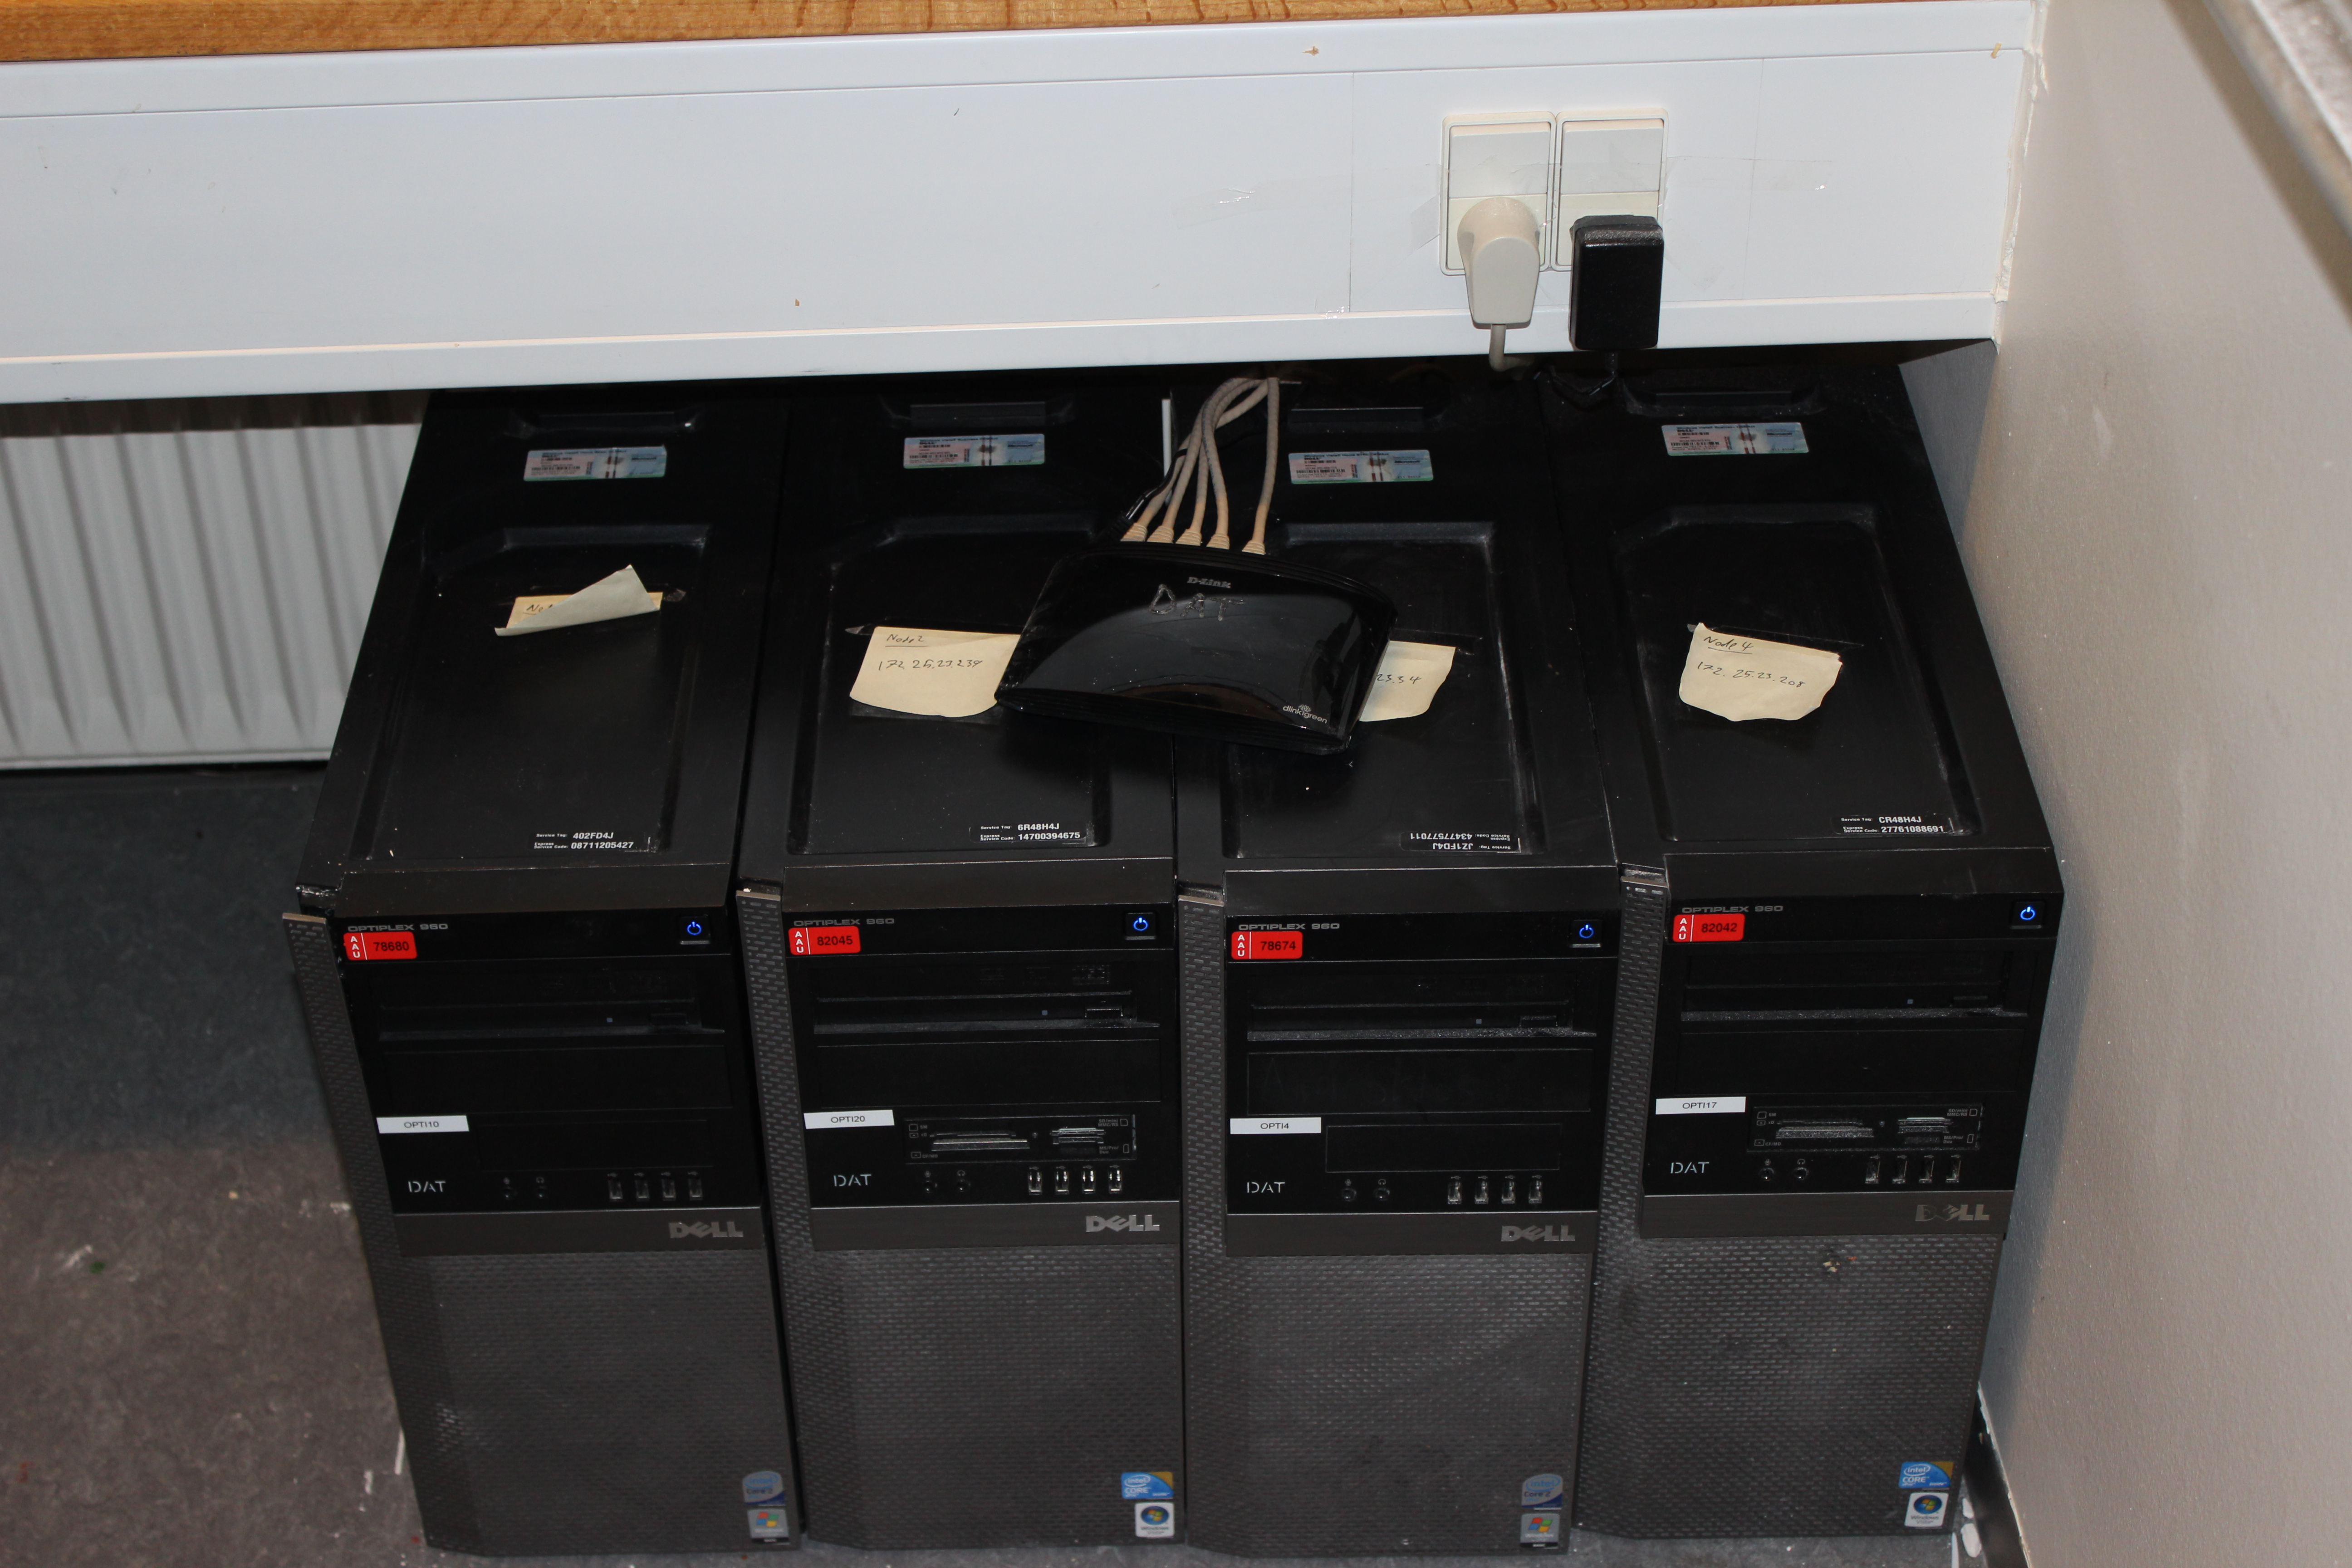
\includegraphics[width=1\textwidth]{img/cluster2.jpg}
  \caption{Physical cluster setup}\label{fig:clustersetup}
\end{figure}

%%% Local Variables:
%%% mode: latex
%%% TeX-master: "../main"
%%% End:
